%%%%%%%%%%%%%%%%%%%%%%%%%%%%%%%%%%%%%%%%%%%%%%%%%%%%%%%%%%%%%%%%%%%%%%%%%%%%%%%
\section{Flujometrías}

De la pirmera iteración se obtuvo la geometría y datos operativos del motor, lo
cual permitió representar la curva de diferencia de presión ($\Delta P$) en
función de la alzada ($l_{v}$) de ambos puertos para diferentes velocidades de
giro, identificando los puntos de mayor interés en los cuales realizar las
flujometrías.
%
Los pares $(l_{v}, \Delta P)$ seleccionados para modelar el flujo del puerto se
detallan en las Figuras~\ref{fig:delta_p_admision} y~\ref{fig:delta_p_escape}.
%
Inicialmente se propusieron 51 flujometrías pudiendo realizar un total de 36
simulaciones que devoliveron 56 valores de $C_{D}$.

\begin{figure}[h]
  \centering
  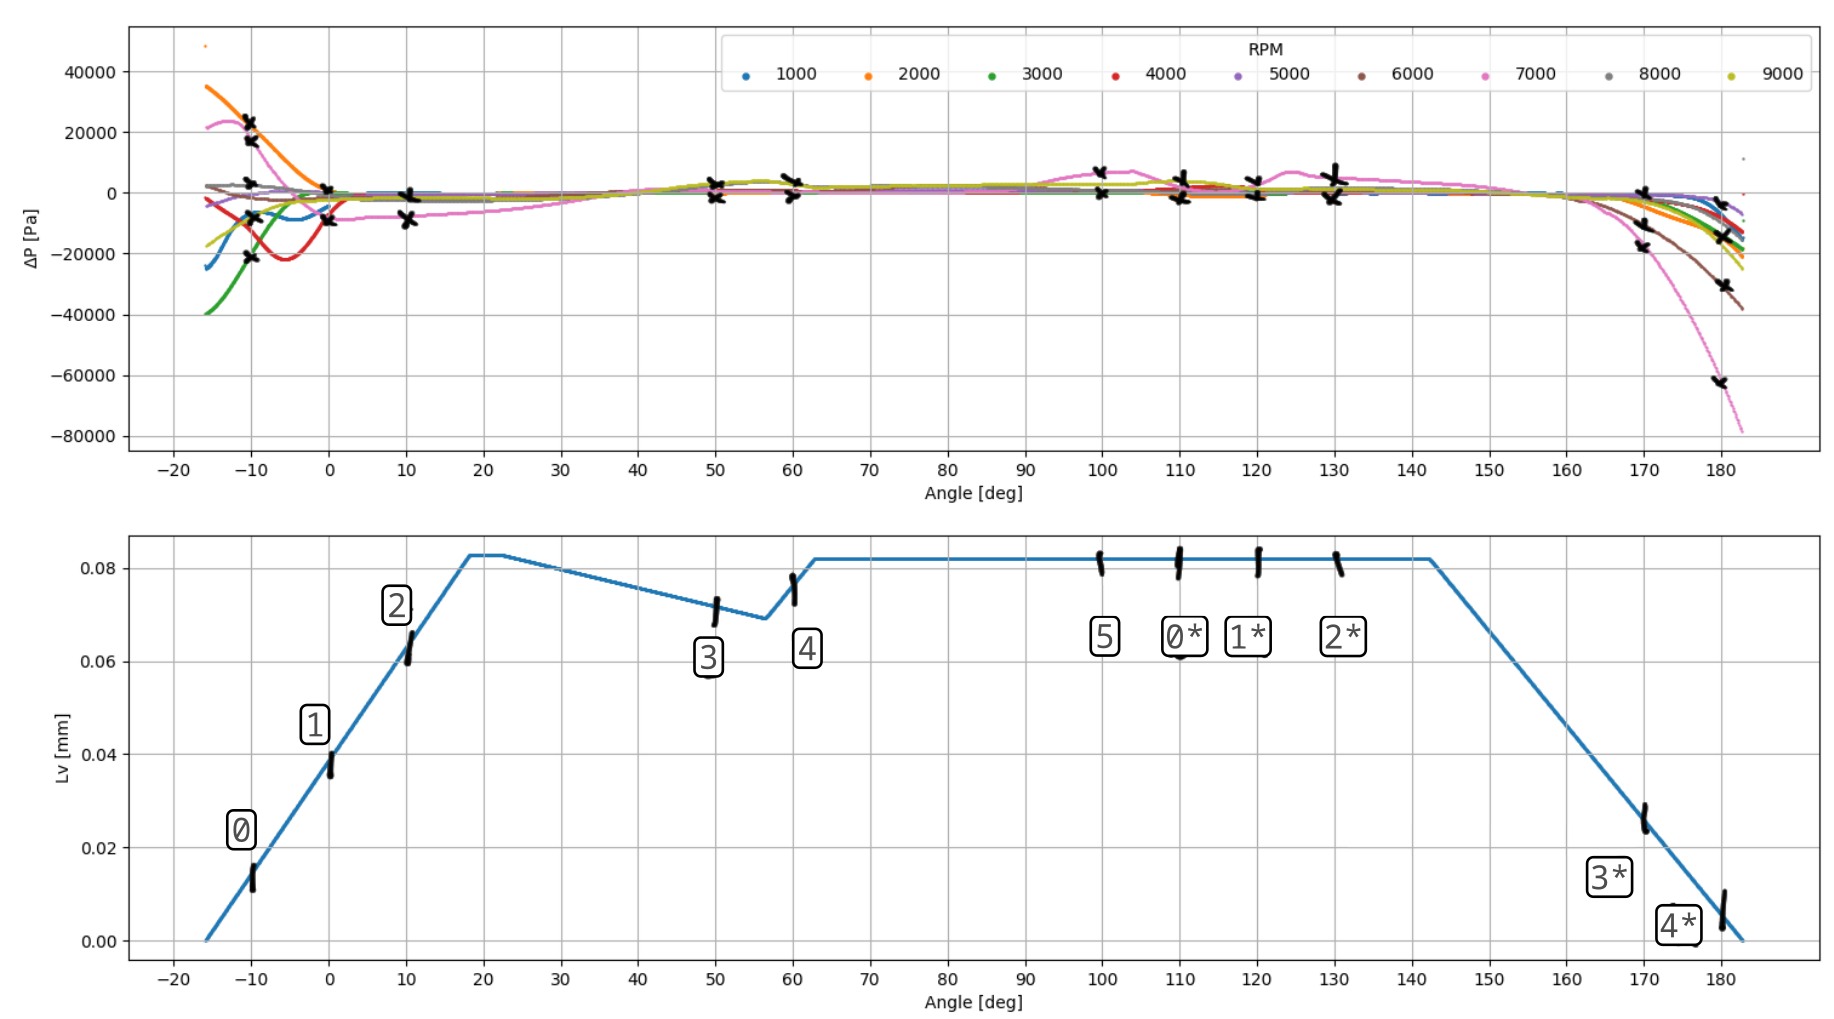
\includegraphics[width=\textwidth]{flujometrias/admision_delta_p_anot.png}
  \caption{Flujometrías puerto de admisión}\label{fig:delta_p_admision}
\end{figure}

\begin{figure}[h]
  \centering
  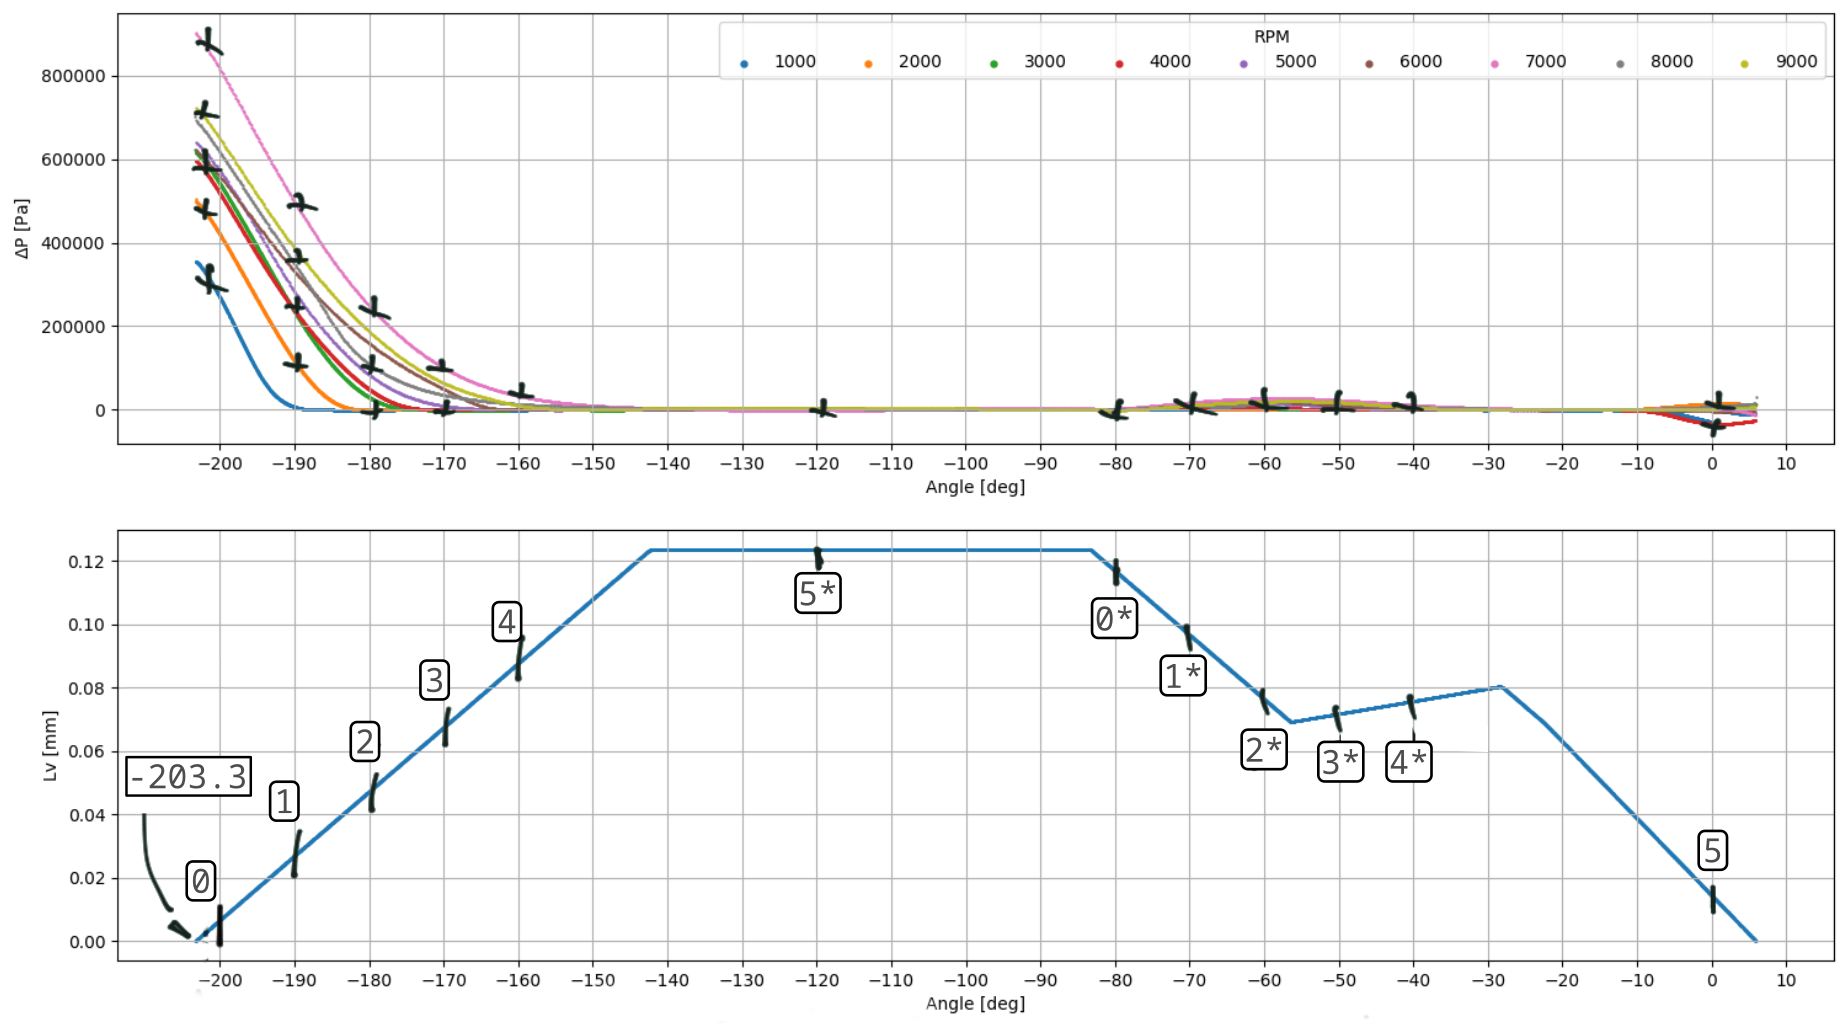
\includegraphics[width=\textwidth]{flujometrias/escape_delta_p_anot.png}
  \caption{Flujometrías puerto de escape}\label{fig:delta_p_escape}
\end{figure}


Algunas flujometrías se realizaron en tres etapas, partiendo de una malla gruesa
con celdas de $15$ mm de tamaño inicial y culminando en celdas de $5$ mm.
%
En otros se realizó directamente la flujometría con mallas base de $5$ mm.

En general se simularon alrededor de $0,02$ segundos de flujo, suficiente para
alcanzar un valor estable del caudal másico, como se indica en la
Figura~\ref{fig:adm_10_7000rpm}, donde se muestra el desarrollo de la simulación
en términos de $\dot{m}$ para el puerto de admisión con el cigüeñal en
$\theta=10^{\circ}$.
%
La línea anaranjada sobre el final de la simulación representa la porción de
datos que se seleccionó para calcular $\dot{m}$, lo cual se realizó tomando la
media de los últimos $n$ valores obtenidos de los resultados de las flujometrías
para los puertos de admisión y escape, las cuales se presentan en el
Anexo~\ref{anexo:1}.
%
La totalidad de puntos evaluados se presentan en las
tablas~\ref{tab:mapa_cd_admision},~\ref{tab:mapa_cd_escape} para el puerto de
admisión y escape respectivamente.

\begin{figure}[ht]
  \centering
  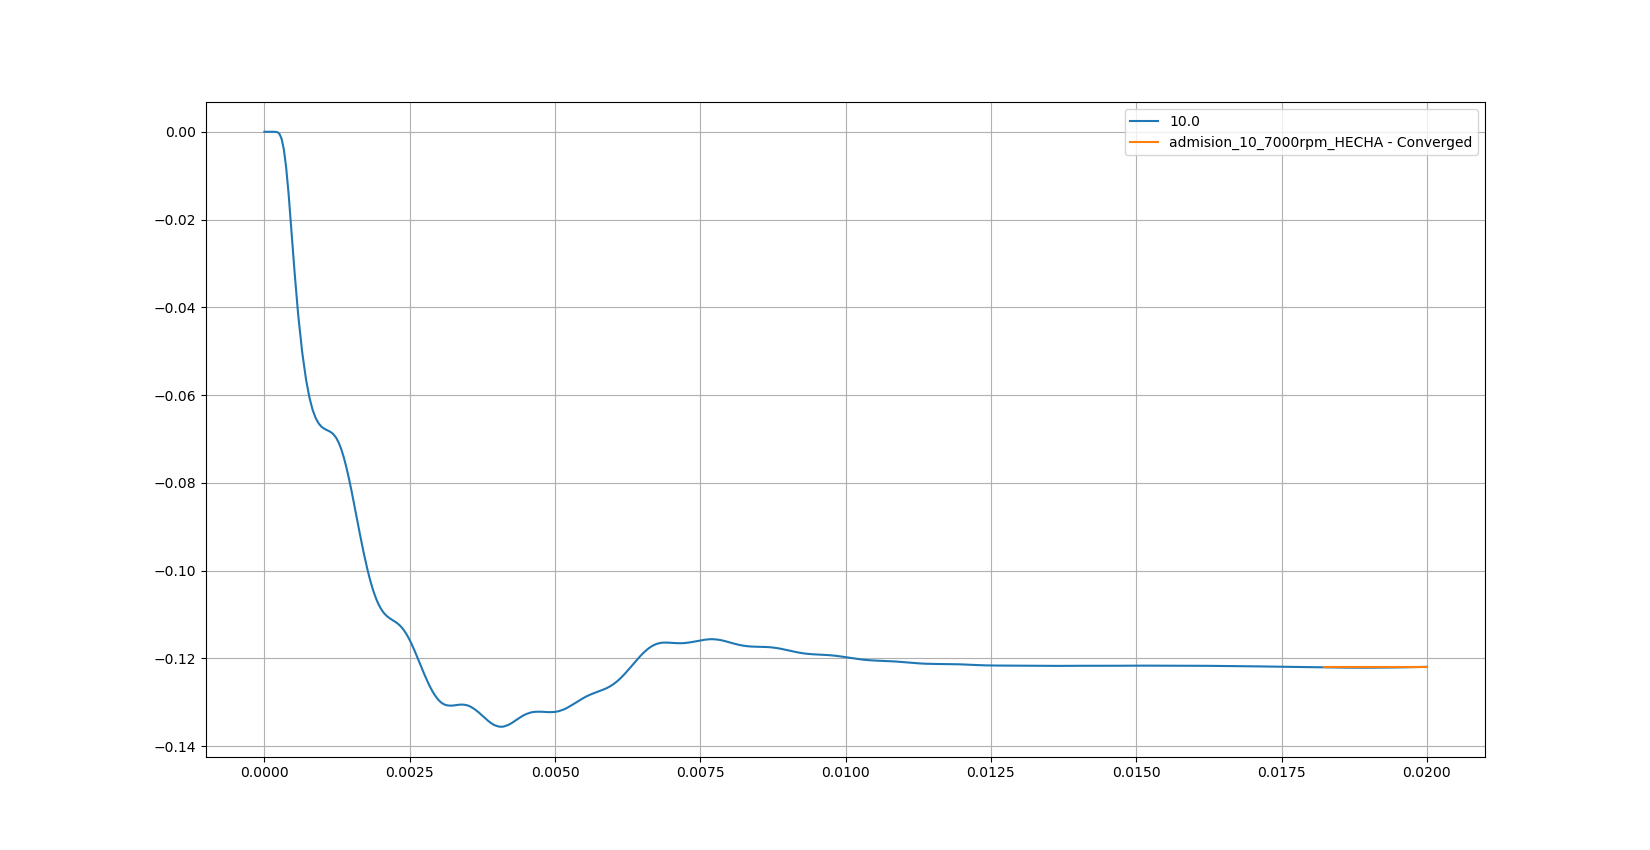
\includegraphics[width=\textwidth]{flujometrias/admision_SFV_10_0.png}
  \caption{Puerto de admisión $10^{\circ}$ \@ $7000$ RPM}\label{fig:adm_10_7000rpm}
\end{figure}

Como se mencionó en la introducción del apartado~\ref{capitulo:DESARROLLO}, la
modificación realizada a ICESym para funcionar con un mapa de $C_{D}$
dependiente de dos variables requiere que los datos de entrada estén
distribuidos en una grilla rectangular.
%
Se utilizo entonces un método de interpolación de punto más cercano suavizado
por promedio móvil con $S=2$ para generar dicha grilla a partir de los puntos
conocidos de $C_{D}$.
%
El resultado puede observarse en las Figuras~\ref{fig:mapa_cd_admision}
y~\ref{fig:mapa_cd_escape}.


\subsection{Puerto de Admisión}
%
En el mapa del coeficiente de descarga para el puerto de admisión se puede
observar en rojo las zonas de menor eficiencia del escurrimiento.
%
%
Esto ocurre para posiciones relacionadas con la apertura y cierre del puerto
donde las presiones y velocidades de flujo involucradas son mayores aumentando
las pérdidas de carga.

En los párrafos siguientes, se definió $\Delta P>0$ cuando el flujo es hacia la
cámara.

\begin{figure}[ht!]
    \centering
    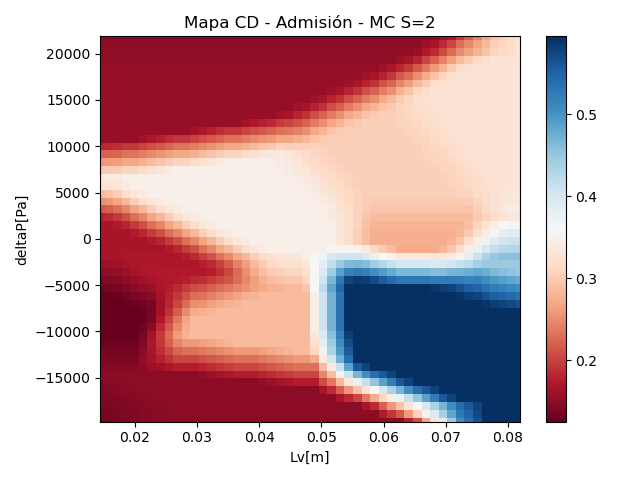
\includegraphics[width=\textwidth]{mapa_cd/mc_s2_mapa_adm.png}
    \caption{Puerto de admisión}\label{fig:mapa_cd_admision}
\end{figure}

\subsubsection{$C_{D}$ máximo}
%
En el mapa del puerto de admisión se observa un máximo de $C_{D,\max}\simeq 0,6$
para para $l_{v}=62,95 mm$ y $\Delta P\simeq -7,37 KPa$, obteniendo un flujo
hacia afuera del puerto de $122,09 g/seg$.
%
Para este caso se observa un reflujo de gases residuales apenas abre el puerto
de admisión, correspondiendo a un ángulo de cigüeñal de $10^{\circ}$ a $7000$
RPM.

La flujometría correspondiente al último instante de la simulación se muetra en
la Figura~\ref{fig:adm_cd_max}.
%
Las líneas de corriente están coloreadas según el módulo de la velocidad y las
flechas indican el sentido de flujo.
%
La mayor velocidad del flujo se da en el gas que sale de la cámara, que
corresponde a masa residual que queda atrapada luego del barrido del puerto de
escape.

\begin{figure}[ht!]
    \centering
    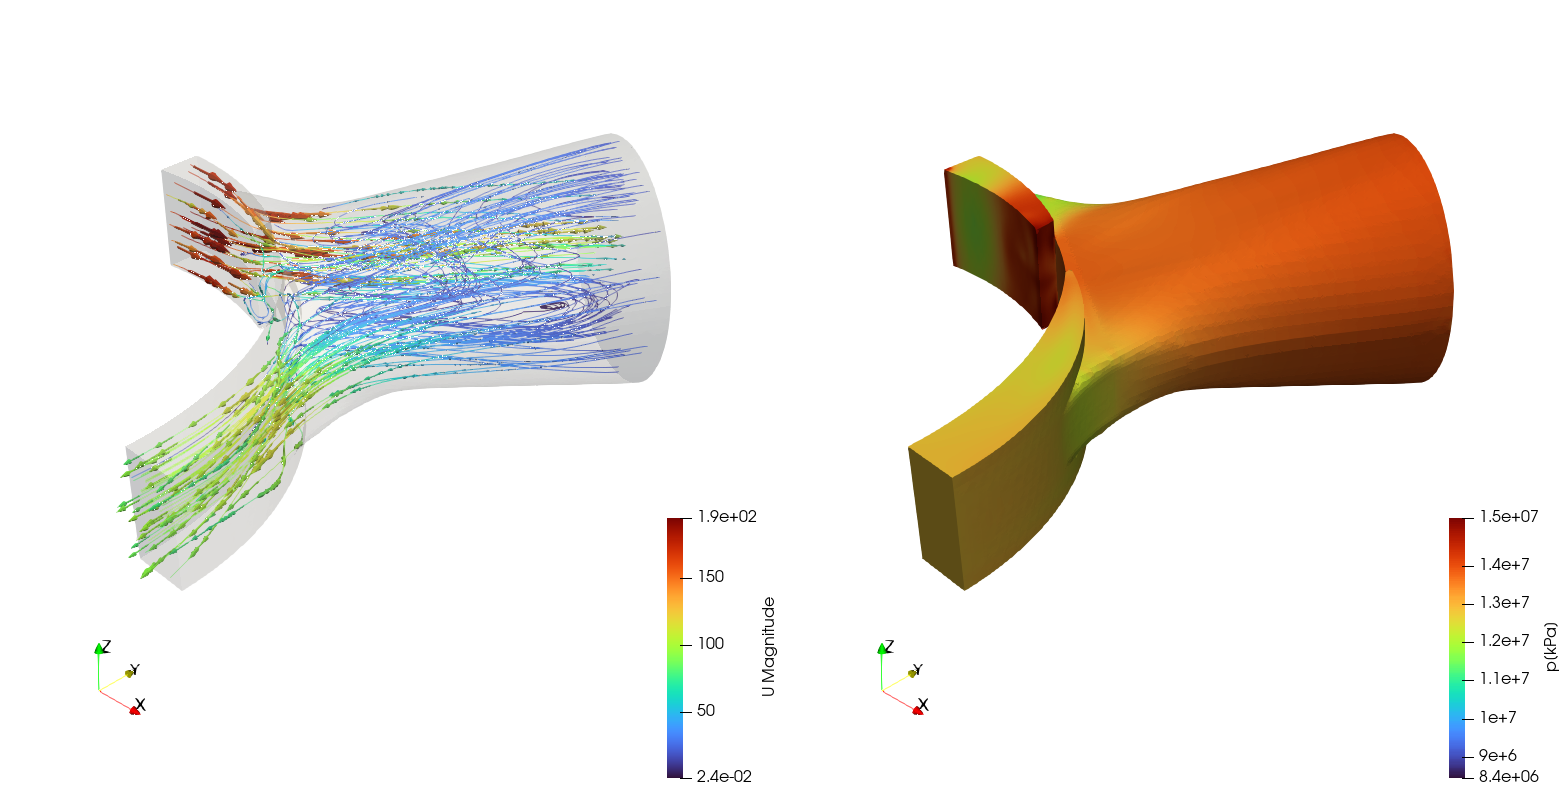
\includegraphics[width=\textwidth]{flujometrias/adm_cd_max.png}
    \caption{Admisión - Valor máximo de $C_{D}$}\label{fig:adm_cd_max}
\end{figure}

\subsubsection{$C_{D}$ mínimo}
%
El menor valor de $C_{D}$ se obtiene para el puerto de admisión en una posición
muy próxima a la apertura, $C_{D,\min}\simeq 0,12$ con un flujo hacia el puerto
de $\dot{m}\simeq 5 g/seg$, $l_{v}=144,3 mm$ y $\Delta P=-6,57 KPa$ para el
puerto a $590^{\circ}$ y $1000$ RPM, ver Figura~\ref{fig:adm_cd_min}.

\begin{figure}[ht!]
    \centering
    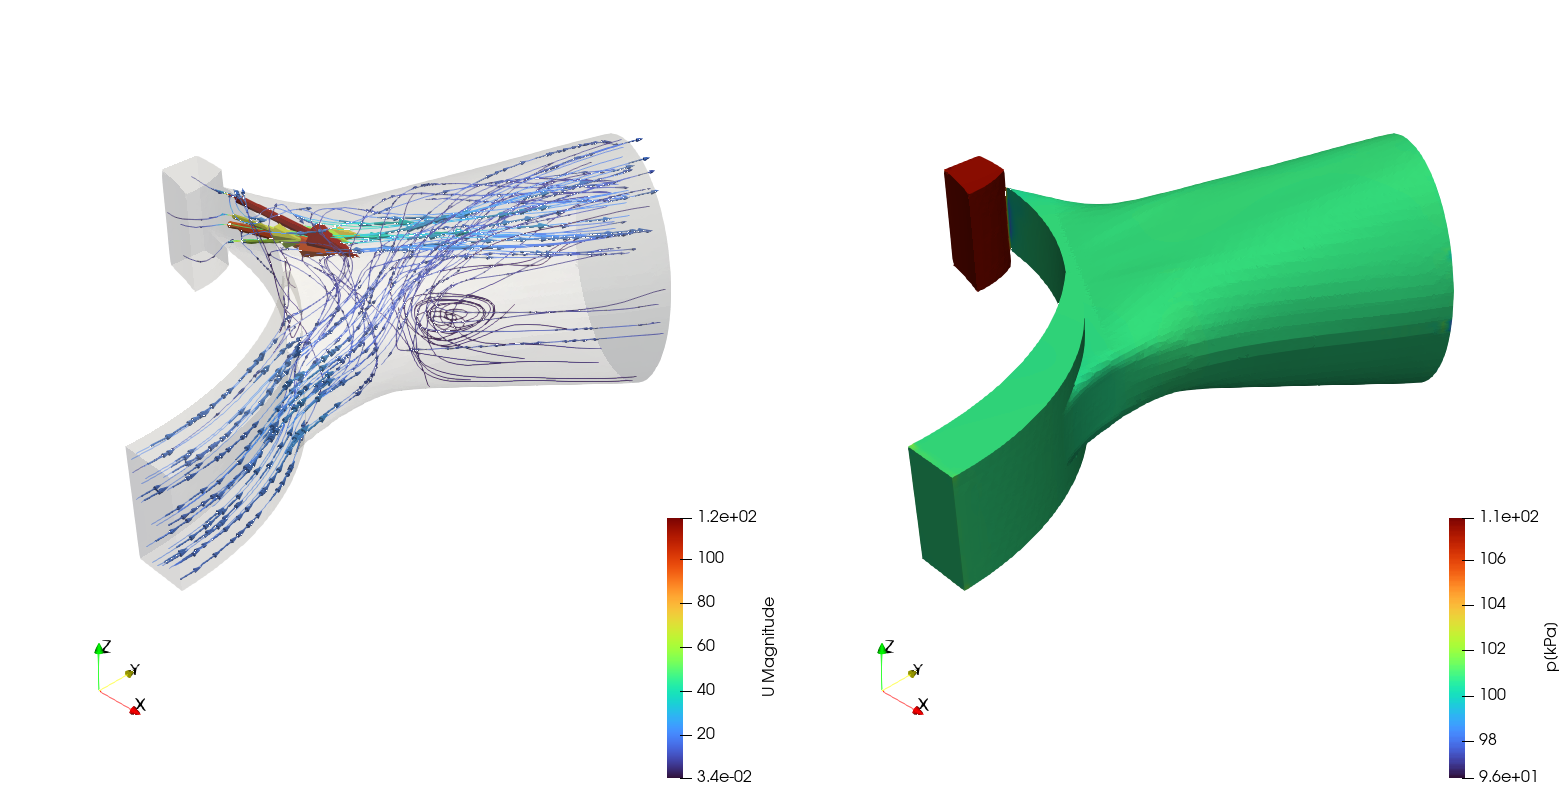
\includegraphics[width=\textwidth]{flujometrias/adm_cd_min.png}
    \caption{Admisión - Valor mínimo de $C_{D}$}\label{fig:adm_cd_min}
\end{figure}

\subsubsection{$\dot{m}$ máximo}
%
En términos de flujo másico, el máximo es $\dot{m}_{\max}\simeq 70 g/seg$ y ocurre
durante un período de máxima apertura del puerto con $l_{v}=81,94 mm$ y
$\Delta P=4,95 KPa$ siendo $C_{D}=0,32874$, ver Figura~\ref{fig:adm_m_max}.

\begin{figure}[ht!]
    \centering
    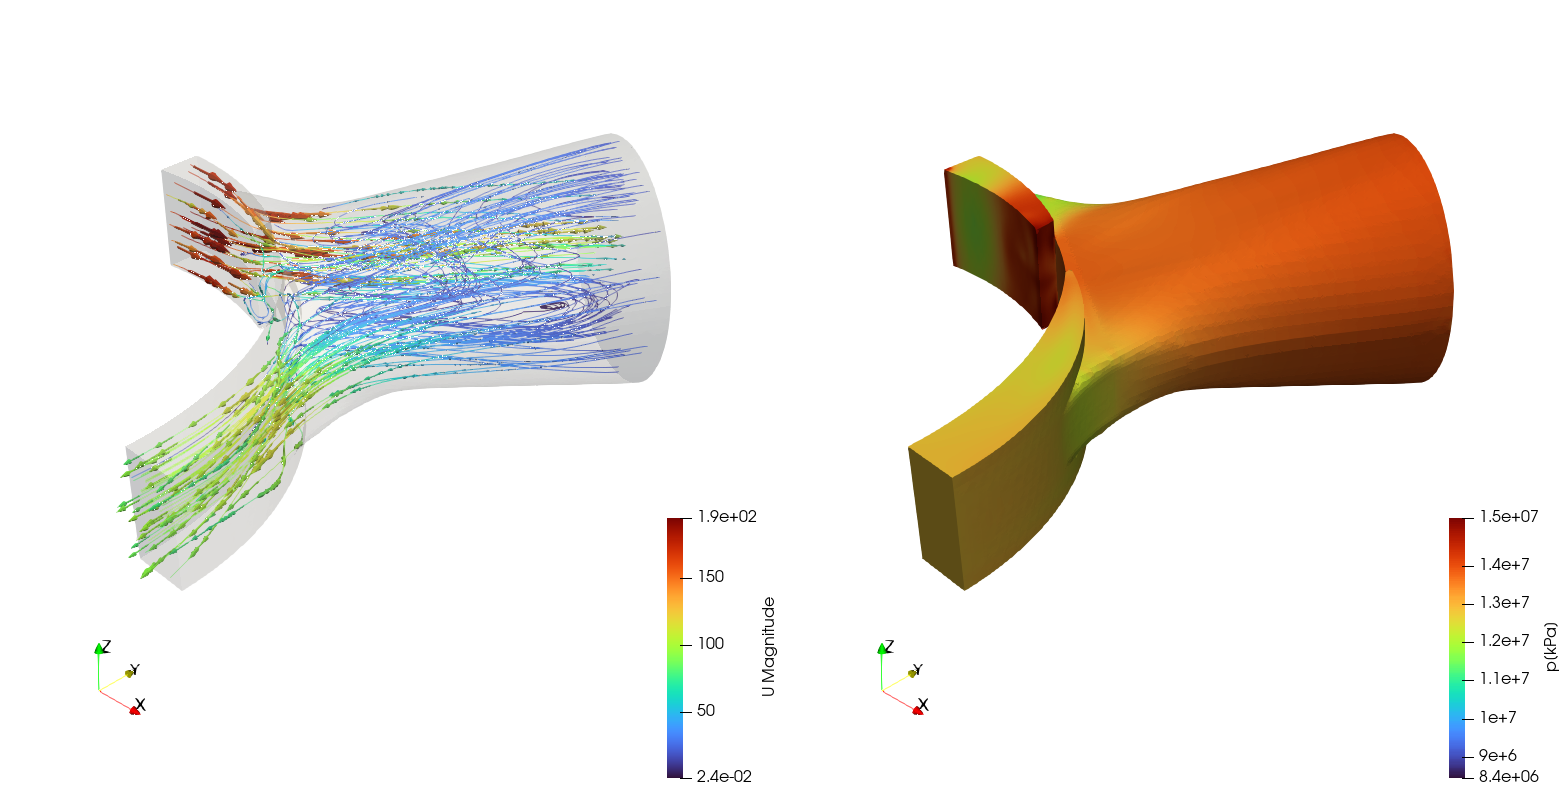
\includegraphics[width=\textwidth]{flujometrias/adm_cd_max.png}
    \caption{Admisión - Valor máximo de $\dot{m}$}\label{fig:adm_m_max}
\end{figure}

\subsection{Puerto de Escape}
%
En la Figura~\ref{fig:mapa_cd_escape} se ilustra el mapa obtenido para el puerto
de escape.
%
La tendencia es similar al puerto de admisión con la diferencia de que no hay
gradientes positivos de presión.
%
La zona con mayores valores de $C_{D}$ corresponde a la máxima apertura del
puerto y valores de presión intermedios.
%

\begin{figure}[ht!]
    \centering
    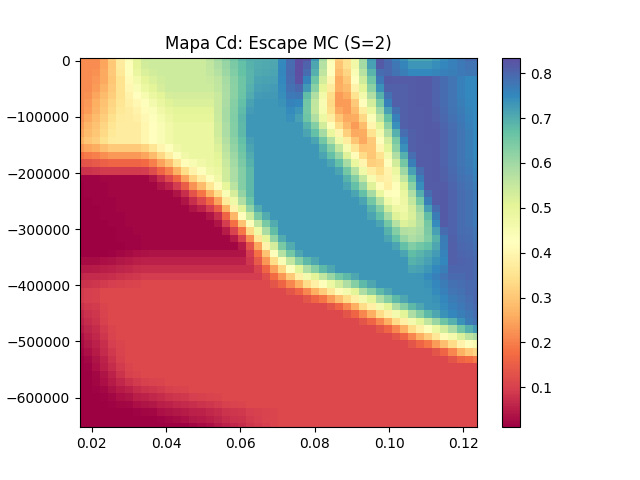
\includegraphics[width=\textwidth]{mapa_cd/mc_s2_mapa_esc.png}
    \caption{Puerto de escape}\label{fig:mapa_cd_escape}
\end{figure}

\subsubsection{$C_{D}$ máximo}
%
Para el puerto de escape se observa el máximo $C_{D,\max}=0,57686$ para
$l_{v}=87,76 mm$, $\Delta P=-1 KPa$ con un flujo másico de $145 g/s$ hacia
afuera para $440^{\circ}$ a $9000$ RPM, ver Figura~\ref{fig:esc_cd_max}.

\begin{figure}[ht]
    \centering
    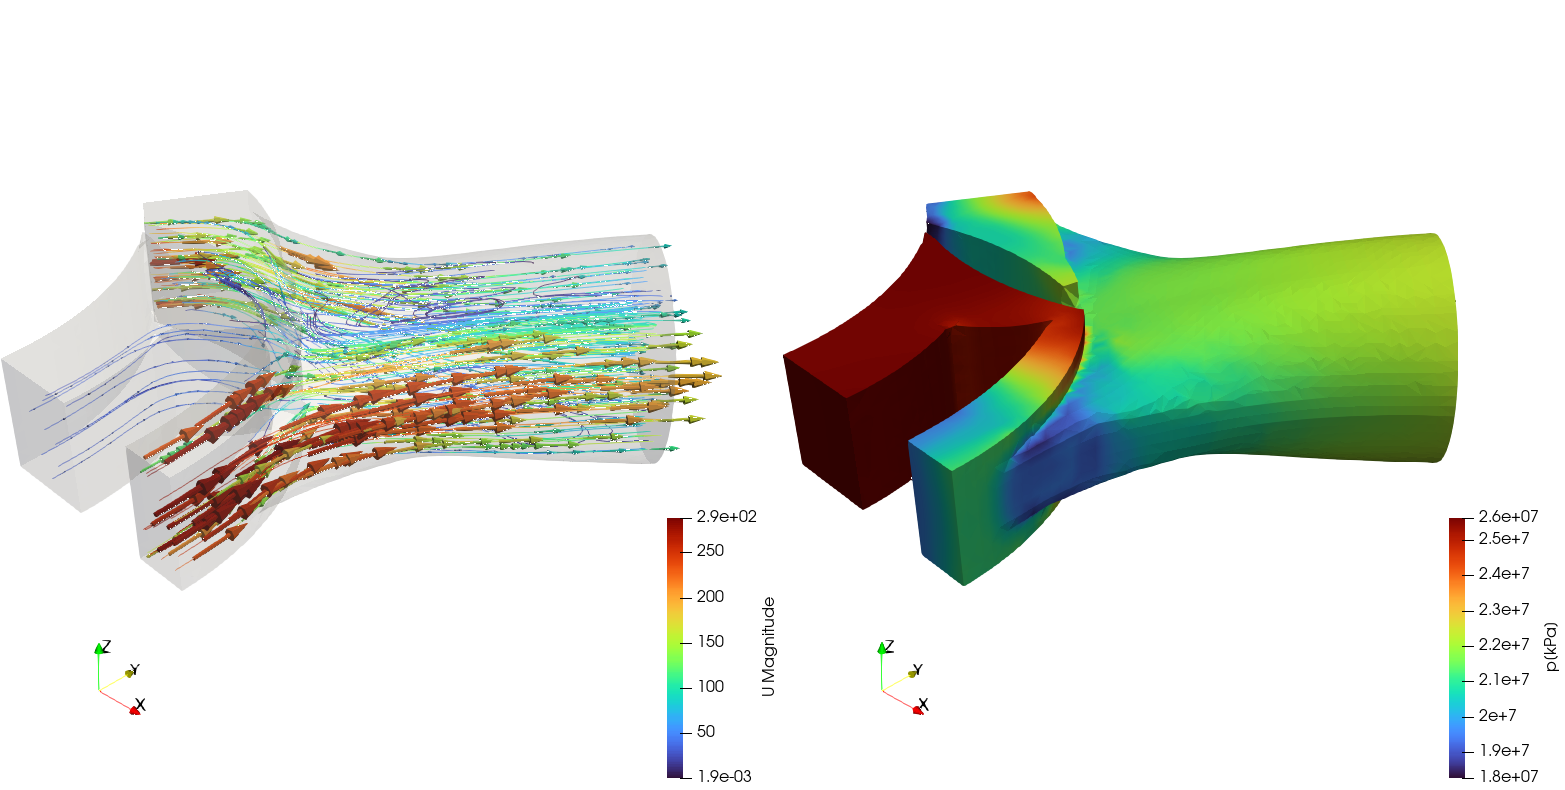
\includegraphics[width=\textwidth]{flujometrias/esc_cd_max.png}
    \caption{Escape - Valor máximo de $C_{D}$}\label{fig:esc_cd_max}
\end{figure}

\subsubsection{$C_{D}$ mínimo}
%
Para $l_{v}=16,83 mm$ y $\Delta P=-652,9 KPa$ se obtiene $C_{D, \min}=0,09631$,
donde el flujo se encuentra bloqueado por la alta diferencia de presión,
alcanzando $\dot{m}=38,6 g/seg$, ver Figura~\ref{fig:esc_cd_min}.

\begin{figure}[ht]
    \centering
    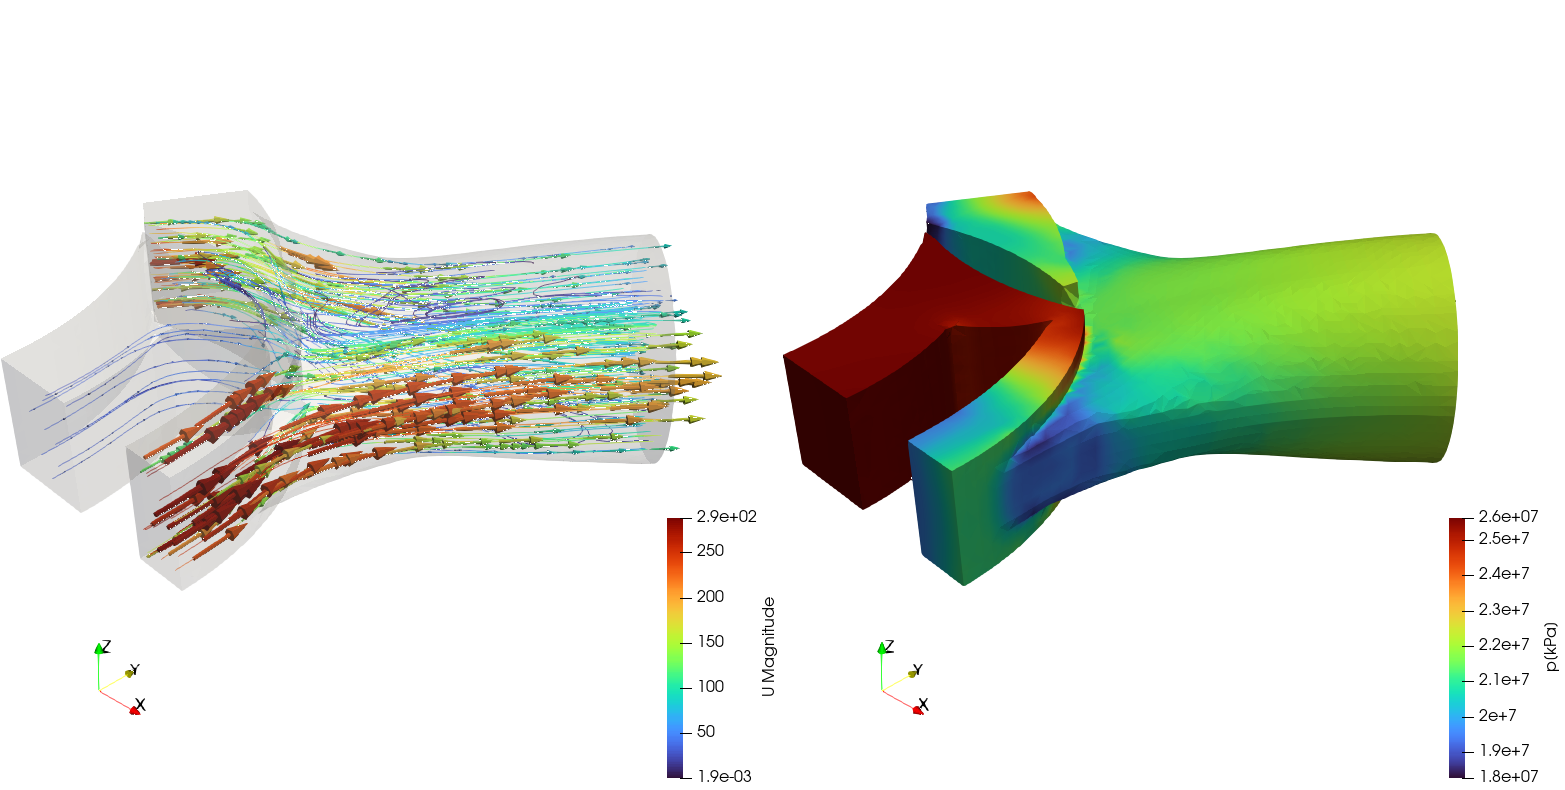
\includegraphics[width=\textwidth]{flujometrias/esc_cd_max.png}
    \caption{Escape - (CAMBIAR POR CD MIN) Valor mínimo de $C_{D}$}\label{fig:esc_cd_min}
\end{figure}

\subsubsection{$\dot{m}$ máximo}
%
El flujo másico máximo es $\dot{m}=176,1 g/seg$ para $l_{v}=87,76 mm$ y
$\Delta P=-334 KPa$, correspondiendo a $440^{\circ}$ y 7000 RPM,
ver Figura~\ref{fig:esc_m_max}.

\begin{figure}[ht]
    \centering
    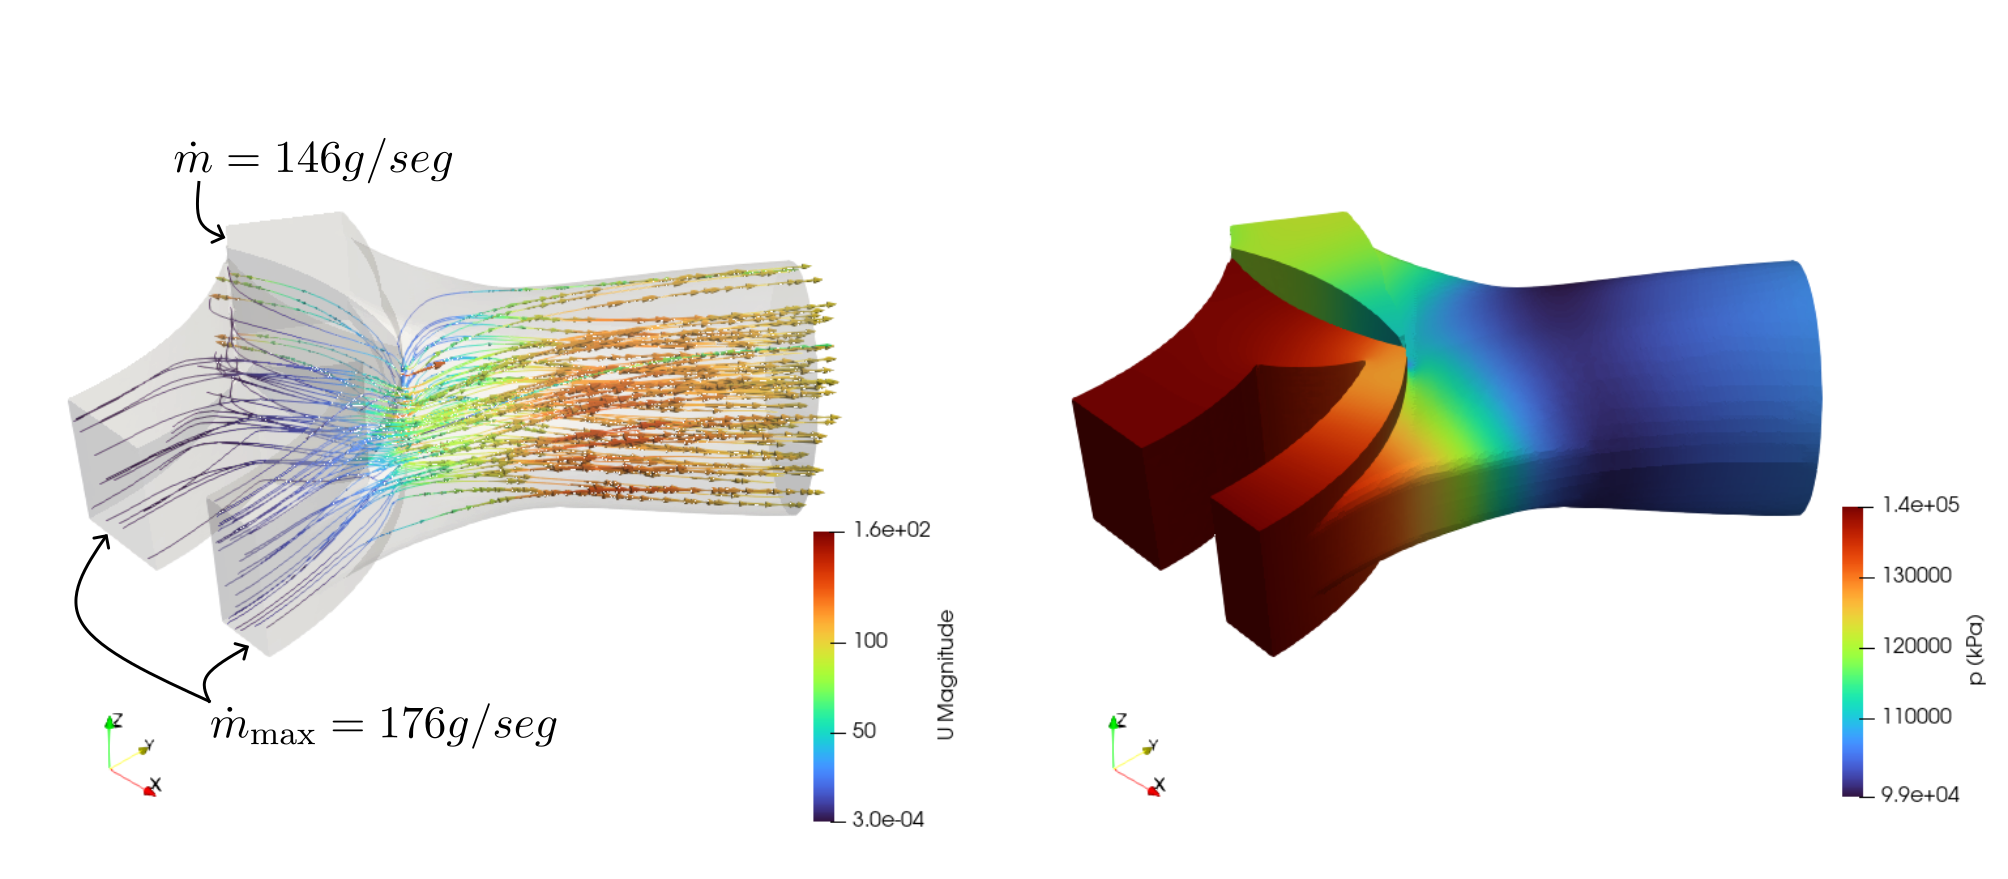
\includegraphics[width=\textwidth]{flujometrias/esc_m_max.png}
    \caption{Escape - Valor máximo de $\dot{m}$}\label{fig:esc_m_max}
\end{figure}
